% !TeX root = ../main.tex
% 原始章节：15-chip-impl-preparation.Rmd

\chapter{芯片实现准备}\label{chap:15-chip-preparation}

\section{各类型IP替换}\label{sec:15-chip-preparation-001}

\subsection{从 FPGA 到芯片}\label{sec:15-chip-preparation-002}

在集成电路设计中，FPGA（现场可编程门阵列）验证环境与流片验证环境存在一定的差异。FPGA
通常用于原型验证和早期开发阶段，而流片后的芯片则是最终产品，两者的设计目标和实现方法有所不同。在从
FPGA 转向芯片的过程中，需要对一些关键的 IP
核进行替换或重新设计，以满足流片环境的需求。

\textbf{FPGA 验证环境与流片验证环境的主要区别}

\begin{enumerate}
\def\labelenumi{\arabic{enumi}.}
\tightlist
\item
  \textbf{硬件结构的不同}:

  \begin{itemize}
  \tightlist
  \item
    \textbf{FPGA}: FPGA
    具有可编程的逻辑单元、可重配置的布线架构和大量内置的 IP 核，如
    PLL、Block RAM 等。这些特性使 FPGA
    非常灵活，能够快速实现和验证复杂的数字电路设计。
  \item
    \textbf{流片芯片}:
    流片后的芯片是经过工艺制造的固定逻辑电路，其结构不可更改，必须在设计阶段完全确定。流片芯片通常对性能、功耗和面积进行优化，这些方面的优化需要针对特定的工艺技术进行。
  \end{itemize}
\item
  \textbf{设计流程的不同}:

  \begin{itemize}
  \tightlist
  \item
    \textbf{FPGA 设计}: FPGA
    设计主要关注功能验证和快速原型实现。设计者可以通过工具链生成位流文件，将设计下载到
    FPGA 上进行验证。这一过程相对快速且灵活，可以频繁迭代修改。
  \item
    \textbf{流片设计}:
    流片设计需要通过一系列复杂的步骤，包括逻辑综合、物理设计、版图生成、时序分析和功耗优化。由于流片成本高昂，设计在进入流片阶段之前必须经过严格的验证和测试。
  \end{itemize}
\end{enumerate}

由于FPGA与ASIC在结构、性能上各不相同，ASIC是基于标准单元库，FPGA用的是厂商提供的宏单元模块，因此首先要进行寄存器传输级(RTL)代码的修改。

\textbf{FPGA 到芯片中需要替换的 IP 核}

在从 FPGA 转向流片芯片的过程中，一些 IP
核需要进行替换或重新设计，以适应流片环境的需求。这些 IP
核包括但不限于以下几个重要组件：

\begin{enumerate}
\def\labelenumi{\arabic{enumi}.}
\item
  \textbf{PLL（Phase-Locked Loop）}:

  数字电路中，时钟是整个电路最重要、最特殊的信号。在ASIC中，用布局布线工具来放置时钟树，利用代工厂提供的PLL进行时钟设计。FPGA中通常已经配置一定数量的PLL宏单元，并有针对时钟优化的全局时钟网络，一般是经过FPGA的特定全局时钟管脚进入FPGA内部，后经过全局时钟BUF适配到全局时钟网络的，这样的时钟网络可以保证相同的时钟沿到达芯片内部每一个触发器的延迟时间差异是可以忽略不计的。因此时钟单元也是需要进行转换的。
\item
  \textbf{Block RAM}:

  存储单元是必须进行代码转换的，ASIC中的存储单元通常用代工厂所提供的Memory
  Compiler来定制，它可以生成.gsp、.v等文件。.v文件只用来做功能仿真，通常不能综合。而最后流片时，只需将标准提供给代工厂。如果直接将FPGA代码中的存储单元作为ASIC的输入，通常综合器是综合不出来的，即使能综合出来，也要花费很长时间，并且资源消耗多、性能不好。因此存储单元要进行代码转换。
\item
  \textbf{Memory Controller}:

  FPGA 中的 Memory Controller 通常使用 IP 核实现，支持多种内存类型，如
  DDR、SRAM 等。在流片设计中，Memory Controller
  需要针对特定的内存类型进行设计，特别是在高速存储器接口设计中，必须确保满足严格的时序和电气性能要求。
\item
  \textbf{其他专用 IP 核}:

  除了上述常见的 IP 核外，其他一些 IP
  核也可能需要替换或定制化设计。例如，寄存器堆、乘法器或其他无法获得代码的FPGA
  IP核。
\end{enumerate}

\subsection{PLL替换}\label{sec:15-chip-preparation-003}

本文以SMIC180工艺库为例介绍相关操作，\textbf{出于学习目的}，该工艺库可从一些网络途径获取。

在FPGA平台，我们一般使用\href{https://www.xilinx.com/products/intellectual-property/clocking_wizard.html}{Clocking
Wizard}
IP来生成不同频率的时钟信号，但在芯片流片时需要使用制造商工艺库中提供的PLL
IP来实现这一功能，本文基于\texttt{S018PLLGS\_LC}介绍如何使用PLL

\textbf{IP引脚定义}

\begin{longtable}[]{@{}
  >{\raggedright\arraybackslash}p{(\linewidth - 4\tabcolsep) * \real{0.1944}}
  >{\raggedright\arraybackslash}p{(\linewidth - 4\tabcolsep) * \real{0.1944}}
  >{\raggedright\arraybackslash}p{(\linewidth - 4\tabcolsep) * \real{0.6111}}@{}}
\toprule\noalign{}
\begin{minipage}[b]{\linewidth}\raggedright
引脚名称
\end{minipage} & \begin{minipage}[b]{\linewidth}\raggedright
输入/输出
\end{minipage} & \begin{minipage}[b]{\linewidth}\raggedright
描述
\end{minipage} \\
\midrule\noalign{}
\endhead
\bottomrule\noalign{}
\endlastfoot
AVDD & 电源 & 专用模拟电源供电 +1.8V \\
AVSS & 地 & 专用模拟地 \\
XIN & 输入 & 来自晶体振荡器或其他时钟源的参考时钟输入 \\
CLK\_OUT & 输出 & 可调输出时钟 \\
TST\_OUT & 输出 & 来自N或M分频器的测试模式输出 \\
N{[}4:0{]} & 输入 & 输入5位分频控制引脚，N{[}0{]}是最低位 \\
M{[}8:0{]} & 输入 & 反馈9位分频控制引脚，M{[}0{]}是最低位 \\
PLL\_TST{[}1:0{]} & 输入 & M和N分频器测试模式\newline{}PLL\_TST{[}1:0{]}=0:0 N分频器测试和正常操作\newline{}PLL\_TST{[}1:0{]}=1:1 M分频器测试\newline{}请在正常模式下将PLL\_TST{[}1:0{]}固定为0 \\
PD & 输入 & 断电控制；高电平有效 \\
OD{[}3:0{]} & 输入 & 输出分频控制引脚 \\
BP & 输入 & 绕过PLL；高电平有效 \\
OE & 输入 & CLK\_OUT使能引脚，高电平有效 \\
\end{longtable}

\textbf{控制信号真值表}

\begin{longtable}[]{@{}lllllll@{}}
\toprule\noalign{}
PD & BP & OE & PLL\_TST\textless0\textgreater{} & PLL\_TST\textless1\textgreater{} & TST\_OUT & CLK\_OUT \\
\midrule\noalign{}
\endhead
\bottomrule\noalign{}
\endlastfoot
0 & 0 & 0 & 0 & 0 & XIN/N & CLK\_OUT \\
0 & 0 & 0 & 1 & 1 & XIN/M & XIN \\
X & 1 & 0 & X & X & 未定义 & XIN \\
X & X & 1 & X & X & 未定义 & 0 \\
其他 & & & & & 未定义 & 未定义 \\
\end{longtable}

\textbf{XIN与CLK\_OUT关系} \[
CLK\_OUT = X_\text{IN} \times \frac{M}{N} \times \frac{1}{NO} \times \frac{1}{2}
\]

\[
M = M_8 \times 256 + M_7 \times 128 + M_6 \times 64 + M_5 \times 32 + M_4 \times 16 + M_3 \times 8 + M_2 \times 4 + M_1 \times 2 + M_0 \times 1 + 2
\]

\[
N = N_4 \times 16 + N_3 \times 8 + N_2 \times 4 + N_1 \times 2 + N_0 \times 1 + 2
\]

\[
N_O = OD3 \times 8 + OD2 \times 4 + OD1 \times 2 + OD0 \times 1
\]

例如：当输入时钟为25MHz，而SoC需要一个133MHz的时钟时，可以按照如下方法定义

% 代码语言：BookSystemVerilog
\begin{CodeBlock}[language=BookSystemVerilog]
S018PLLGS_LC SOC_PLL(
  .XIN(clk_25m),
  .CLK_OUT(soc_clk),
  .N(5'b0_0001),
  .M(9'b0_0001_1110),
  .PLL_TST(2'b00),
  .RESET(1'b0),
  .PD(1'b0),
  .OD(4'b0001),
  .BP(1'b0),
  .OE(1'b0)
);
\end{CodeBlock}

此时\(M = 32, N = 3, NO = 1,CLK_{-}OUT=25 \times \frac{32}{3} \times \frac{1}{1} \times \frac{1}{2} = 133.\dot 3(MHz)\)

\subsection{SRAM替换}\label{sec:15-chip-preparation-004}

在FPGA中，我们一般使用Block Ram
IP或XPM宏来实现SRAM，在流片过程中则需要将这些SRAM替换为目标工艺库中的IP，我们需要使用制造公司提供的SRAM生成器来生成我们所需的SRAM。本文以
SMIC 0.18um Dual-Port Memory Compiler为例。

官方提供的安装包包括如下文件：

\begin{longtable}[]{@{}
  >{\raggedright\arraybackslash}p{(\linewidth - 2\tabcolsep) * \real{0.2055}}
  >{\raggedright\arraybackslash}p{(\linewidth - 2\tabcolsep) * \real{0.7945}}@{}}
\toprule\noalign{}
\begin{minipage}[b]{\linewidth}\raggedright
名称
\end{minipage} & \begin{minipage}[b]{\linewidth}\raggedright
作用
\end{minipage} \\
\midrule\noalign{}
\endhead
\bottomrule\noalign{}
\endlastfoot
S018DP.jar & 存储器生成器应用程序 \\
S018DP.csh & C Shell 设置文件 \\
S018DP\_ug.pdf & 用户手册 \\
S018DP.notes & 发布说明 \\
Library & GDS Smart Option 库，用于处理 GDS 文件并执行各种智能操作 \\
\end{longtable}

S018DP.csh文件内容如下

% 代码语言：BookShell
\begin{CodeBlock}[language=BookShell]
setenv MC_INSTALL_PATH `pwd`
java -jar S018DP.jar&
\end{CodeBlock}

运行该脚本可启动生成器的GUI界面

界面如图\ref{fig:sram-gen}所示：

\begin{figure}[htbp]
  \centering
  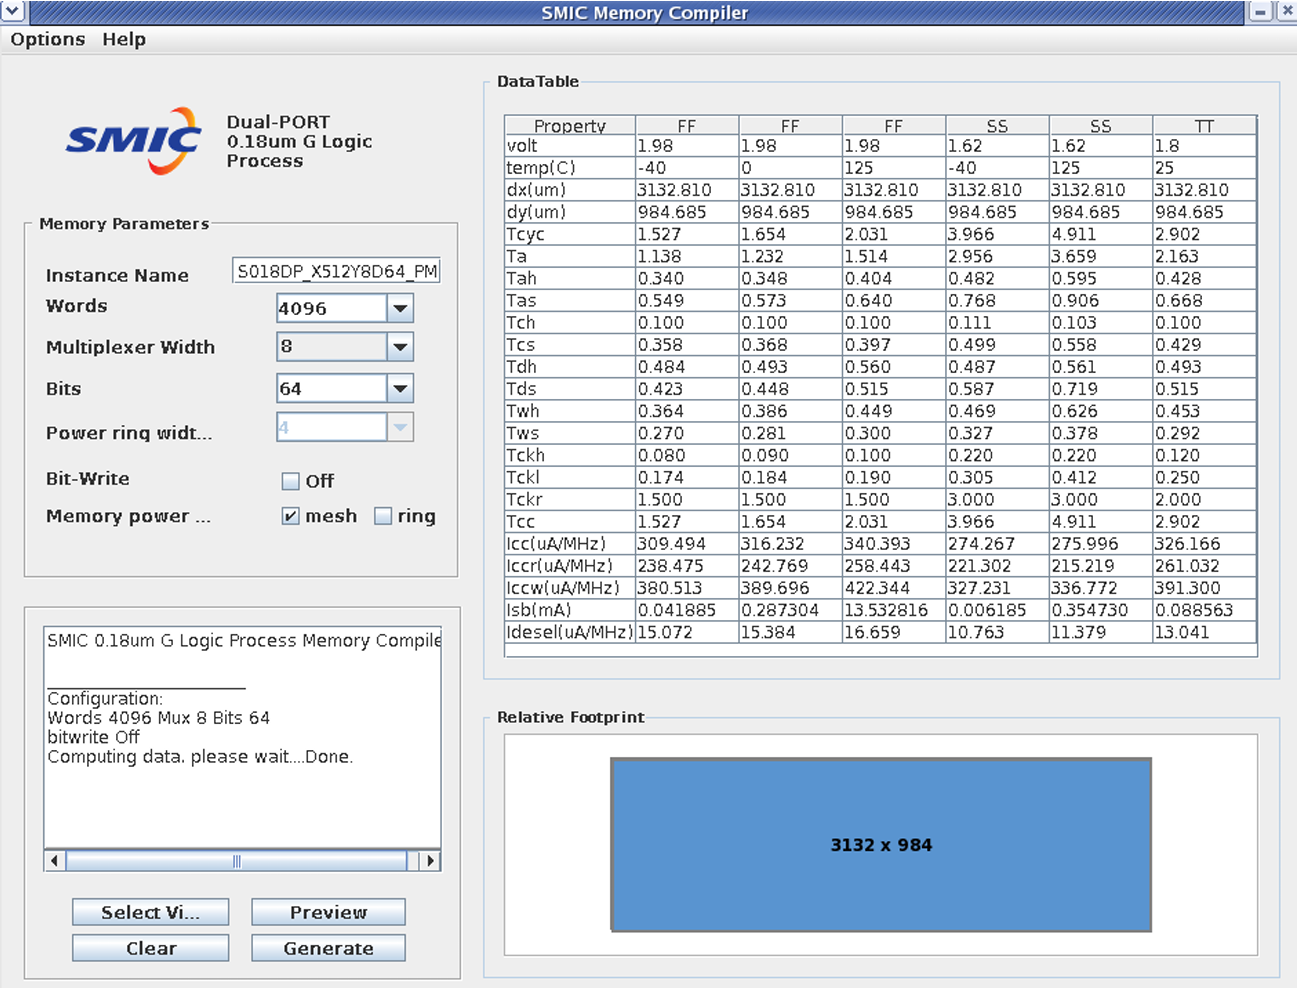
\includegraphics[width=1\linewidth]{assets/15/sram-gen.png}
  \caption{SRAM生成器GUI}
  \label{fig:sram-gen}
\end{figure}

\begin{enumerate}
\def\labelenumi{\arabic{enumi}.}
\item
  Memory Parameters（存储器参数）

  存储参数（Memory
  Parameters）面板包含输入字段和复选框。您可以通过从每个参数对应的下拉子菜单中选择所需的值或在输入字段中输入值来更改``字（Word）''、``多路复用器（Multiplexer）''和``位（Bits）''的值。此外，您还可以在复选框中选择``位写入（Bit-Write）''的开关状态（on/off）以及电源结构的``网格（mesh）''或``环形（ring）''选项。如果选择``环形''，则``电源环宽度''的下拉子菜单将变为可选状态，并且需要适当地设置电源环的尺寸，考虑到芯片级电源分配方法、电源环的数量、宽度和供电线连接的位置以及电流消耗。

  当您完成参数值的填写后，可以点击``预览（Preview）''按钮查看更新后的数据表面板（DataTable）、消息（Message）面板和相对占位面积（Relative
  Footprint）面板。例如，您可以为具有8192个字、64位和16多路复用器宽度的特定实例生成视图。在``字''下拉子菜单中选择8192，在``多路复用器宽度''下拉子菜单中选择16，在``位''下拉子菜单中选择64。然后点击``预览''按钮，数据表面板、消息面板和相对占位面积面板将会更新。
\item
  Relative Footprint （相对占位面积）

  相对占位面积面板显示了相应特定实例的纵横比。当您更改记忆参数并点击``预览''按钮后，相对占位面积将会更新。
\item
  Data Table （数据表）

  数据表显示了相应特定实例的拐角、布局尺寸、时序、电流和功耗信息。当您更改记忆参数并点击``预览''按钮后，数据表将会更新。
\item
  Message（信息）
  消息面板在您生成实例时显示相关消息。消息包括正在生成的实例的配置信息、正在生成的视图类型信息以及成功生成的提示信息。当您输入的值超出预定范围时，消息面板还会报告问题。
\end{enumerate}

当然也可以使用脚本生成：

% 代码语言：BookShell
\begin{CodeBlock}[language=BookShell]
#!/bin/bash
rm -rf *~
rm -rf *_RAM_DP_*
HEAD=S018DP

# words, bits, mux
config=(
'128 128 4'
'128 128 1'
'1024 16 4'
'1024 32 4'
'256 128 1'
'256 16 2'
'512 64 2'
'128 128 1'
)

for i in "${config[@]}"; do
  row=($i)
  W=${row[0]}
  B=${row[1]}
  M=${row[2]}
  RAM_NAME=${HEAD}_RAM_DP_W${W}_B${B}_M${M}
  echo $RAM_NAME
  rm -rf $RAM_NAME
  mkdir $RAM_NAME
  java -jar S018DP.jar -words $W -mux $M -bits $B -v -lib -pdf -gds -cdl -mbist -lef -powermesh -savepath ./$RAM_NAME -instname $RAM_NAME
\end{CodeBlock}

\subsection{SDRAM 控制器介绍}\label{sec:15-chip-preparation-005}

SDRAM控制器是一种用于控制同步动态随机存储器(SDRAM)的硬件设备。它能够实现高速、可靠的内存读写操作，并经常用于计算机、通讯系统和其他嵌入式应用中。SDRAM控制器有着复杂的内部工作机制，通过其内部的逻辑电路，实现对SDRAM存储器芯片的精细控制。

一个SDRAM控制器通常包含读写控制器、地址发生器、时钟控制器和数据缓冲等组件。它能够识别读取和写入命令，并控制存储器的读取和写入操作的执行时间。在操作过程中，SDRAM控制器先将外部指令和数据传输到数据缓冲区，然后再基于内部时钟更新SDRAM存储器中的数据。此外，SDRAM控制器还通过检测数据总线的情况，实现对数据的检查和纠错，以提高内存数据的可靠性。

SDRAM控制器的内部时钟频率非常高，通常达到百兆赫兹甚至更高。它能够对存储器按照指定的工作模式进行读写操作，如CAS时序、预充电和自刷新等。此外，SDRAM控制器还可以支持多通道、多控制器和多级缓存等高级特性，以大幅提高系统读写效率。

LainChip项目选定的内存控制器是SpinalHDL项目中的\href{https://github.com/SpinalHDL/SpinalHDL/tree/dev/lib/src/main/scala/spinal/lib/memory/sdram}{Sdram}库。SpinalHDL是一个高级的硬件描述语言，其以Scala语言为基础，提供一套框架，通过使用现代编程范式，打破了常用
HDL
中许多降低开发效率的限制。SpinalHDL项目中的Sdram控制器提供了AXI总线到SDRAM接口的翻译功能。该控制器分为前端与后端两部分，前端部分将AXI请求翻译为SDRAM的目标状态，后端根据前端传送的目标状态向SDRAM芯片发送对应的指令。该控制器支持AXI总线的突发传输特性，因此能进行较高速率的数据传输。

\section{EDA工具环境搭建}\label{sec:15-chip-preparation-006}

本节主要针对芯片实现过程中使用的EDA工具进行介绍，主要介绍所使用的工具类别及功能、流程等，并对照一些实际的脚本来参考如何使用EDA工具。

\subsection{EDA工具概览}\label{sec:15-chip-preparation-007}

芯片实现流程如下图\ref{fig:chip-flow}所示，其中每一步都会有对应的EDA工具来进行相应的操作，总体可分为前端设计与仿真、前端综合与评估、后端实现及验证三个部分。下面根据流程中常用的EDA工具按顺序进行一个简单的介绍（其中FPGA验证在第十二章已经描述，这里不再进行阐述）。

\begin{figure}[htbp]
  \centering
  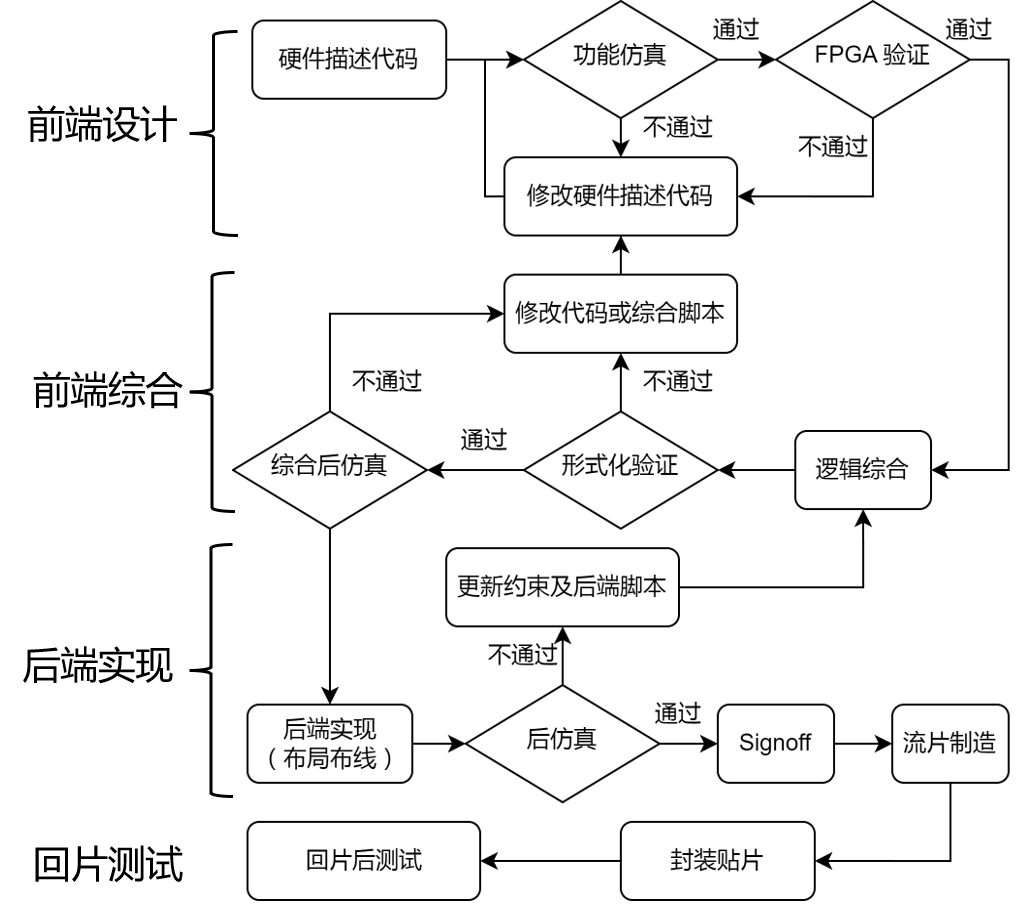
\includegraphics[width=0.5\linewidth]{assets/15/芯片设计流程.png}
  \caption{芯片设计流程示意图}
  \label{fig:chip-flow}
\end{figure}

\begin{enumerate}
\def\labelenumi{\arabic{enumi}.}
\tightlist
\item
  \textbf{芯片前端设计与仿真工具}：
\end{enumerate}

\begin{itemize}
\tightlist
\item
  \emph{Matlab}：在复杂的大型芯片项目中，往往前端设计还会涉及系统架构设计，通过matlab等首先对架构进行建模与评估，对整体设计划分模块。
\item
  \emph{VSCode}：在设计好架构之后就会通过硬件描述语言编写RTL代码（在本教材中除了VerilogHDL还有更抽象的Chisel等硬件描述语言来编写RTL），编写工具使用编辑器即可。
\item
  \emph{ModelSim}：是Mentor Graphics公司（先为Siemems
  EDA一部分）开发的一种高性能、交互式和可扩展的HDL仿真工具。
\item
  \emph{VCS}：全称为Verilog Compiled
  Simulator，是Synopsys公司推出的一款高性能、高容量的硬件描述语言（HDL）仿真工具。它主要用于验证数字集成电路（IC）设计，包括在寄存器传输级（RTL）和门级上的验证。
\item
  \emph{Iverilog}：全称为Icarus
  Verilog，是一个轻量级跨平台开源Verilog仿真软件，一般配合开源波形查看工具GTKWave配合使用。
\end{itemize}

\begin{enumerate}
\def\labelenumi{\arabic{enumi}.}
\setcounter{enumi}{1}
\tightlist
\item
  \textbf{芯片前端综合与评估工具}：
\end{enumerate}

\begin{itemize}
\tightlist
\item
  \emph{DC}：全称为Design
  Compiler，是Synopsys公司推出的用于芯片逻辑综合的工具。具体为将高抽象层级描述（寄存器传输级，RTL）转化为低层次的门级网表的工具，以实现电路逻辑功能的综合与优化等，并可以得到一个评估的时序、功耗、面积等。
\item
  \emph{PT}：全称为PrimeTime，是Synopsys公司推出的用于芯片静态时序分析的工具。具体功能为确保电路在时钟信号作用下能正确采样和保持数据，以及相较于DC工具更为全面的时序检查。一般在前端综合过后会使用PT工具进行更进一步的静态时序分析。在后续做完后端详细布线、提取参数后将生成的SPEF文件发送给PrimeTime获取更准确的STA分析结果。
\item
  \emph{PTPX}：全称为PrimeTime PX，是Synopsys公司推出的用于功耗分析的工具。
\item
  \emph{Formality}：Synopsys推出的用于形式验证的工具。主要功能为对综合后的网表与HDL设计进行对比，验证功能上的等价性，以保证逻辑综合过程没有改变HDL所描述的电路功能。
\end{itemize}

\begin{enumerate}
\def\labelenumi{\arabic{enumi}.}
\setcounter{enumi}{2}
\tightlist
\item
  \textbf{芯片后端实现与验证工具}：
\end{enumerate}

\begin{itemize}
\tightlist
\item
  \emph{Innovus}：Cadence公司推出的芯片后端实现的布局布线工具，即将逻辑综合后生成的门级电路通过物理方式连接起来，形成具有制造意义的版图的过程。
\item
  \emph{StarRC}：Synopsys推出的用于寄生参数提取的工具。
\item
  \emph{Voltus}：是一款Cadence公司推出的用于电源完整性分析和优化的EDA工具。
\item
  \emph{Calibre}：是Mentor公司推出的用于物理验证的EDA工具，对芯片版图进行检查，以确保其符合制造工艺和性能要求。具体包括设计规则检查（DRC）、版图与原理图一致性检查（LVS）、电气规则检查（ERC）等。
\end{itemize}

下面将针对这三种类别的EDA工具进行展开描述。

\subsection{芯片前端设计及仿真工具}\label{sec:15-chip-preparation-008}

首先编写HDL代码需要一个易用的代码编辑器，推荐使用\emph{VSCode}，因为其有较多的插件可以在代码设计的前期就检查到语法等方面的错误，也便于编辑代码。
在编写完成后需要对代码进行功能测试，测试工具包括\emph{VCS}、\emph{ModelSim}等，这里主要针对\emph{VCS}进行介绍与流程描述。

\emph{VCS}可支持多种抽象级别的仿真，包括行为级、RTL级、门级、SignOff等，这使得其可以支持芯片流程中的多个位置的仿真（前端RTL仿真到后端版图后仿真等）。\emph{VCS}工作原理分为两个阶段：编译和仿真。编译阶段，工具将Verilog/SystemVerilog源代码转换为中间表示形式，并生成可执行文件（通常为simv）。仿真阶段，通过执行这个可执行文件，对设计进行仿真，模拟这个运行过程并输出仿真结果。

具体的流程为：

\begin{itemize}
\item
  准备阶段：准备好Verilog源代码、testbench测试文件以及其他测试数据等相关文件。并创建一个file.list文件用于列出所有需要编译的Verilog文件路径，以方便后续使用VCS命令编译。
\item
  编译阶段：使用VCS命令编译，命令格式如下：
\end{itemize}

% 代码语言：BookShell
\begin{CodeBlock}[language=BookShell]
vcs -full64 -sverilog -debug_access+all -f file.list -timescale=1ns/1ns -l com.log
\end{CodeBlock}

其中，-full64表示在64位模式下编译，-sverilog表示支持SystemVerilog语言，-debug\_access+all用于保存调试过程中生成的各种文件，-f
file.list指定file.list文件作为输入，-timescale=1ns/1ns定义仿真时间单位，-l
com.log用于保存编译日志。

编译完成后，会生成一个名为simv的可执行文件（使用-o选项可以指定其他名字）。

\begin{itemize}
\tightlist
\item
  仿真阶段：在命令行中，通过执行simv文件来启动仿真，执行命令的基本格式如下：
\end{itemize}

% 代码语言：BookShell
\begin{CodeBlock}[language=BookShell]
./simv -l run.log
\end{CodeBlock}

仿真完成后，可以通过testbench中的\$display语句或其他输出方式查看仿真结果。此外，还可以使用VCS提供的图形化界面（如DVE）来观察波形和仿真结果。

\begin{itemize}
\tightlist
\item
  波形查看：在testbench中，可以通过添加下述语句调用dump
  fsdb函数来生成FSDB波形文件。例如：
\end{itemize}

% 代码语言：BookVerilog
\begin{CodeBlock}[language=BookVerilog]
initial begin  
  if ($test$plusargs("dumpfsdb")) begin  
    $fsdbDumpfile("TEST.fsdb");  
    $fsdbDumpvars(0, top_tb);  
  end  
end
\end{CodeBlock}

上述代码具体含义为：当检查仿真启动命令参数包含字符dumpfsdb时，将top\_tb模块及其所有子模块的信号进行转储为TEST.fsdb文件。之后使用Veridi查看波形，编译配置Veridi后打开上述.fsdb波形文件即可查看。

对于使用\emph{VCS}进行门级仿真，只需要将逻辑综合生成的网表文件（生成verilog）替换原来的RTL代码文件（若启用SDF反标，则执行类似下述命令）：

% 代码语言：BookShell
\begin{CodeBlock}[language=BookShell]
vcs -full64 -sverilog -sdf -max/typ/min:inst_name:sdf_path -debug_access+all -f 
file.list -timescale=1ns/1ns -l com.log
\end{CodeBlock}

其中max/typ/min选择一个，是指启用SDF文件中指定的最小值、典型值、最大值的一种，在实例inst\_name上进行反标时序。

\subsection{芯片前端综合与评估工具}\label{sec:15-chip-preparation-009}

在代码功能验证过后，将代码进行逻辑综合以将RTL设计转换成门级网表。\emph{DC}是Synopsys综合工具，内嵌了多种工具用于将RTL转化为网表并根据时序、面积等约束进行收敛。这里首先介绍\emph{DC}的使用流程，再用一个简单的脚本来说明\emph{DC}的具体使用过程。

\emph{DC}的使用流程：

\begin{itemize}
\tightlist
\item
  启动与环境初始化：可使用命令行启动与图形界面启动两种方式，启动过程需要读取初始化文件，用于初始化工具环境、库环境、工作路径等。
\item
  指定库文件：使用set target\_library来指定目标库、使用set
  link\_library来指定链接库等。工艺库由代工厂提供，如中兴国际SMIC180nm库等。
\item
  读入设计文件：使用read命令或analyze\&elaborate组合命令读入设计文件（如Verilog或systemVerilog文件，此时DC将设计文件转换成中间格式（如GTECH格式），便于后续处理。
\item
  施加设计约束：定义设计约束，包括面积约束、时序约束、DRC（设计规则检查）约束等；时序约束如定义时钟（create\_clock）、设置输入输出延迟（input\_delay、output\_delay）等；DRC约束如最大转换时间、最大扇出负载、最大负载电容等。
\item
  定义设计环境：设置工艺参数（如温度、电压等）和I/O端口属性（如负载、驱动、扇出等）；这些参数将影响设计综合及优化结果。
\item
  选择编译策略：DC进行优化的目的是权衡时序与面积，以满足用户对功能、速度、面积等要求。编译策略可选择compile与compile\_ultra（需要单独的license）两种。可添加high-effort指令来使DC更加努力达到所约束的目标。
\item
  输出文件：包括输出网表文件、报告文件等。报告包括时序报告、面积报告以及功耗报告等。用户可以根据输出报告来分析电路中可能存在的问题。
\end{itemize}

下面给出一个简化的\emph{DC}使用流程示例命令与脚本（假设已经由一个RTL设计文件design.v以及基本库文件stdcells.db、io\_cells.db等）：

bash文件：

% 代码语言：BookShell
\begin{CodeBlock}[language=BookShell]
#!/bin/bash  
  
# 设置环境变量，这里需要根据实际情况替换路径  
export SYNOPSYS_SIM_SETUP=/path/to/synopsys/setup_files  
# 注意：这通常是csh或tcsh脚本，如果是bash环境可能需要调整 
source $SYNOPSYS_SIM_SETUP/synopsys_dc_setup.csh   
  
# 切换到工作目录  
cd /path/to/your/working/directory  
  
# 清理之前的运行结果（可选）  
rm -rf csrc work report* *.db *.log *.vpd *.v *.sdf  
  
# 启动DC（这里以命令行模式为例，也可以启动design_vision图形界面）  
dc_shell -f run_dc.tcl  
\end{CodeBlock}

run\_dc.tcl文件，假设上述bash脚本与该文件在同一目录下：

% 代码语言：BookTcl
\begin{CodeBlock}[language=BookTcl]
# 设定工作库  
set_app_var search_path "+/path/to/std_cells_lib +/path/to/io_cells_lib"  
  
# 读取设计文件  
read_verilog -library WORK design.v  
  
# 定义库和链接库  
link  
  
# 设置目标库  
set target_library "typical.db"  
  
# 设置综合策略  
set_synthesis_strategy -effort high  
  
# 设置时钟  
create_clock -name clk -period 10 [get_ports clk]  
  
# 设置输入输出延迟（示例）  
set_input_delay -clock clk 3 [all_inputs]  
set_output_delay -clock clk 3 [all_outputs]  
  
# 编译设计
compile -map_effort high  
  
# 检查时序  
check_timing  
  
# 如果需要，可以导出网表和其他文件  
write_file -format verilog -hierarchy flat -output design_synth.v  
write_sdf -version 2.1 design.sdf  
  
# 结束DC会话（可选，通常在脚本末尾自动完成）  
exit
\end{CodeBlock}

一些实现过程根据需要配置，该脚本只是给出一个简单的示例。其他工具例如Formality等使用较为简单，这里不再详细阐述。

\subsection{芯片后端实现与验证工具}\label{sec:15-chip-preparation-010}

后端实现包括布局布线（也称为物理实现physical
design）、时序signoff、功耗与IR
signoff、物理验证等过程。这里主要针对芯片物理实现使用的EDA工具\emph{Cadence
Innovus}进行描述。

\emph{Cadence
Innovus}是一款高性能的电子设计自动化（EDA）工具，专为集成电路（IC）的物理设计和实现而开发。它主要用于大规模集成电路（VLSI）的布局布线，能够处理从RTL到GDSII的整个设计流程。Innovus具有强大的并行处理能力，支持现代节点的复杂工艺，并且能够优化功耗、性能和面积（PPA）。

具体的设计流程为：

\begin{itemize}
\tightlist
\item
  导入设计：包括综合生成的网表文件、库文件、IO约束文件等。
\item
  Floorplanning：定义芯片的总体结构和宏模块布局，确定芯片各部分的相对位置。
\item
  Placement：自动将标准单元放置到芯片平面上，同时考虑到信号延迟、功耗和面积等因素，自动调整单元位置执行放置优化。
\item
  时钟树综合（CTS）：设置并插入时钟树，确保所有时钟域内部的时钟信号能够同步达到。
\item
  布线（Routing）：执行全芯片的信号布线，并优化布线以减少信号延迟和交叉干扰（crosstalk）。
\item
  功耗分析与优化：分析芯片的动态与静态功耗，通过调整电压、频率或布局来优化功耗。
\item
  设计优化：针对性能、功耗和面积进一步优化，应用工程变更订单（ECO）进行最后的修正。
\end{itemize}

\section{仿真模拟与性能评估环境搭建}\label{sec:15-chip-preparation-011}

在集成电路（IC）设计过程中，仿真模拟和性能评估是验证设计符合预期要求的关键步骤。环境搭建需要精心规划，以确保仿真结果的准确性和可靠性。

\subsection{前仿与后仿}\label{sec:15-chip-preparation-012}

前仿（Pre-simulation）：指在实际物理实现之前对设计进行的仿真。通常在逻辑设计阶段（如RTL设计）进行。目的是验证设计在逻辑层面是否正确，检查功能是否符合预期。使用硬件描述语言（如Verilog或VHDL）编写的设计，在EDA工具（如ModelSim,
VCS等）中运行。可以使用波形查看器进行深入分析。

后仿（Post-simulation）：在设计的物理实现（如布局布线后）进行的仿真。使用的是更接近实际制造条件的数据。目的是验证物理实现是否影响了设计的功能，确认时序和性能指标。利用抽取出的布线信息和寄生参数（通过工具如StarRC），在EDA仿真工具中进行更接近真实条件的仿真。

\subsection{测试验证环境搭建}\label{sec:15-chip-preparation-013}

合适的测试平台和工具是设计验证的关键，仿真工具可以使用 Verilator 或 VCS。Verilator 是一种开源的硬件仿真器，主要用于将 Verilog 代码编译成 C++ 或 SystemC 代码，从而实现高效的仿真。它的设计目标是进行更快的仿真速度，而非完全的功能仿真; VCS 是 Synopsys 公司开发的一款商业级仿真器，广泛应用于芯片设计的各个阶段。它支持完整的 Verilog 和 SystemVerilog 语言，包括设计和验证的所有特性。VCS 能够进行精确的时序仿真、功耗分析、代码覆盖率报告等，适用于从功能验证到最终时序验证的各个阶段。波形查看工具可以采用 GTKWave，GTKWave 是一个开源的波形查看工具，主要用于查看数字电路仿真生成的波形数据。它支持多种仿真工具的输出格式，广泛用于硬件设计和验证过程中，帮助设计者分析仿真结果。

在完成处理器初步设计后，可以根据 \url{https://github.com/BUAA-CI-LAB/eula-env} 中的 README 接入 Eula-Env 集成芯片敏捷开发平台，其中可通过 Difftest 框架分析处理器执行周期、指令条数、IPC 等指标。

测试用例：开发一系列详尽的测试用例来覆盖所有可能的设计场景。这些测试用例应该旨在揭露功能缺陷和性能瓶颈。Eula-Env 中 AM 内置部分常用测试，例如功能测试、Coremark、Dhrystone 测试，同时包括 Linux 系统仿真，可以对处理器进行较为完善的测试。若需额外编写测试，可参考 \url{https://github.com/BUAA-CI-LAB/am/blob/master/README.md} 中关于创建单源/多源文件程序的介绍。

自动化测试：为了提高效率和准确性，应尽可能自动化测试过程。可使用 Python、Tcl、CI/CD 来控制仿真流程，自动化数据收集和结果分析。
